% ============================================================================
% Crystal Explorer -- ACDSA 2027 submission
%
% Built on the standard IEEEtran conference class, which is what ACDSA's
% "conform to IEEE format" requirement is based on. Before final submission,
% download the OFFICIAL ACDSA LaTeX template (acdsa.org/submission ->
% ACDSA_latex.rar) and:
%   1. Diff its .cls/.sty files against stock IEEEtran -- swap the
%      \documentclass line and any custom package below if they differ.
%   2. Add the conference header the CFP requires at the RIGHT of the first
%      page (see the commented \AddConfHeader example near \begin{document}).
%   3. Remove/replace any manual page numbering (ACDSA requires none from
%      authors -- IEEEtran's conference mode already omits it by default).
% ============================================================================
\documentclass[conference]{IEEEtran}
\IEEEoverridecommandlockouts

\usepackage{cite}
\usepackage{amsmath,amssymb,amsfonts}
\usepackage{graphicx}
\usepackage{textcomp}
\usepackage{xcolor}
\usepackage{booktabs}
\usepackage{url}
\usepackage[hidelinks]{hyperref}

\def\BibTeX{{\rm B\kern-.05em{\sc i\kern-.025em b}\kern-.08em
    T\kern-.1667em\lower.7ex\hbox{E}\kern-.125emX}}

\begin{document}

\title{Crystal Explorer: A Python-based Pipeline for Protein Crystallization Conditions}

\author{
\IEEEauthorblockN{1\textsuperscript{st} Ruth Nana Njantang}
\IEEEauthorblockA{\textit{Research and Technology Institute (RIT)} \\
\textit{Area Science Park} \\
34149 Trieste, Italy \\
ORCID: \href{https://orcid.org/0000-0002-0785-0916}{0000-0002-0785-0916}}
\and
\IEEEauthorblockN{2\textsuperscript{nd} Andrea Dalle Vedove}
\IEEEauthorblockA{\textit{Elettra Sincrotrone Trieste S.C.p.A} \\
34149 Basovizza, Trieste, Italy \\
andrea.dallevedove@elettra.eu}
\and
\IEEEauthorblockN{3\textsuperscript{rd} Valerio Piomponi}
\IEEEauthorblockA{\textit{Research and Technology Institute (RIT)} \\
\textit{Area Science Park} \\
34149 Trieste, Italy \\
valerio.piomponi@areasciencepark.it}
\thanks{This project has been funded by the European Union -- NextGenerationEU
within the projects: NFFA-DI cod.\ IR0000015 and EFC cod.\ SSU2024-00002
through Area Science Park, Trieste.}
}

\maketitle
\pagestyle{plain}

\begin{abstract}
Choosing a starting crystallization condition for a new protein target is still largely a trial-and-error process, even though the Protein Data Bank (PDB) already contains the successful conditions of hundreds of thousands of previously solved structures. This information is locked inside \texttt{pdbx\_details}, a free-text field written by depositors in inconsistent, non-standardized phrasing, which makes it unusable for large-scale automated retrieval. We present Crystal Explorer, a python-based Django web application that turns a single query sequence into a structured set of crystallization cocktails mined from its closest X-ray-solved homologs. The system runs a four stage pipeline: (1) an RCSB sequence similarity search restricted to X-ray structures, with per-hit metadata retrieval; (2) a curated dictionary and regex-based extraction of reagents and concentrations from \texttt{pdbx\_details}, covering 354 canonical reagents and 1{,}180 lexical variants; (3) grouping of homologous hits into unique conditions with interactive (Plotly) and static (Matplotlib/PDF) pH-vs-temperature and pH-vs-PEG visualizations; and (4) generation of FAIR-compliant, JSON-LD metadata for every output artifact. In this work, the system's architecture and methodology are illustrated with a real run on the SARS-CoV-2 papain-like protease (PLpro). We further evaluate the compound extractor itself on two independent panels of 10{,}000 real \texttt{pdbx\_details} entries each, mined by the pipeline from 30\%-sequence-identity clusters of the PDB that share no protein family and no entry with each other; a random 1{,}000 entries of each panel were audited by hand. The first panel served as a development set whose errors were then fixed; the second, a held-out test of the fixed and frozen extractor, reaches 99.3\% precision and 94.2\% recall (F1 0.967) over 2{,}898 verified reagent mentions, with 84.6\% of entries extracted without a single error. The remaining misses are mostly ligands and rare reagents absent from the dictionary, an open long tail no fixed dictionary fully closes. Crystal Explorer is released under the MIT license at
\url{https://github.com/RitAreaSciencePark/Protein_Crystallization_Data_Extraction}.
\end{abstract}

\begin{IEEEkeywords}
protein crystallization, crystallization conditions, Protein Data Bank, text mining, FAIR data, structural biology, data extraction, web application
\end{IEEEkeywords}

% ============================================================================
\section{Introduction}

Crystallization is usually the bottleneck step in determining the three-dimensional structure of a macromolecule by X-ray diffraction. One
of the central difficulties is setting up cocktails that produce a single crystal suitable for data collection~\cite{kwon2013modeling}; no
comprehensive theoretical framework yet guides this process, and success depends on bringing the macromolecule to a supersaturated state without disrupting its native conformation~\cite{mcphersoncudney2014optimization}. Because the relevant variables are numerous and 
broad, crystallization is typically approached by screening an extensive trial matrix and refining successive rounds~\cite{luft2014crystallization,mcpherson2014introduction}; a condition that succeeds for one protein guaranties nothing for another.
A more targeted starting point is available in principle: the PDB already documents the exact crystallization cocktail for every X-ray structure ever deposited~\cite{berman2000pdb,burley2021rcsb}, and a new target sharing sequence similarity with an existing structure inherits that homolog's conditions as a strong empirical prior.

In practice, this prior is very hard to use at scale. The relevant field, \texttt{exptl\_crystal\_grow.pdbx\_details}, is unstructured free text written independently by tens of thousands of depositors, so the same reagent appears under dozens of spellings, abbreviations, and unit conventions (e.g.\ ``PEG 3350'', ``peg3350'', ``polyethylene glycol 3,350''), and concentrations are expressed inconsistently or omitted entirely - a documented obstacle to mining crystallization data at archive scale~\cite{kirkwood2015analysis}. Manually reading this text for even a handful of homologs does not scale, and the PDB's search interface returns entries, not structured chemistry. Existing curated resources address part of this problem but as static, query-independent snapshots, and a complementary line of machine learning work predicts whether a sequence is likely to crystallize \emph{at all} without prescribing a condition, neither closes the gap between ``here is my sequence'' and ``here is a shortlist of cocktails worth trying''.

This paper presents \textbf{Crystal Explorer}, a python-based web application and
underlying pipeline that closes that gap end to end. Given a protein (or nucleic acid) sequence, it: (i) finds X-ray-solved homologs via RCSB's sequence search API, built on the
MMseqs2~\cite{steinegger2017mmseqs2,steinegger2019userguide} aligner,
at orders of magnitude higher throughput than the PDB's traditional
BLAST-based tools~\cite{altschul1990basic,donkor2014bioinformatics};
(ii) parses the free-text crystallization conditions of every hit into
structured (reagent, concentration) pairs using a curated chemical
dictionary and a tiered regex matcher; (iii) groups hits sharing the
same condition, rendering interactive and static pH-vs-temperature and
pH-vs-PEG plots and a summary table cross-referenced by a shared row
identifier; and (iv) emits FAIR-compliant~\cite{wilkinson2016fair},
 metadata for every output file. The whole pipeline runs from
a single web form and results page, with a history of past searches and
an in-page 3D structure viewer, so no command-line experience is
required.

Our contributions are:
\begin{itemize}
  \item An open, reproducible pipeline that converts unstructured PDB
        crystallization metadata into structured, analysis-ready data,
        using a 354-reagent / 1{,}180-alias curated chemical dictionary mined
        from real deposition text.
  \item A grouping and traceability scheme (a shared \texttt{row\_id}) that
        keeps every plotted point, PDF table row, and interactive web-table
        row linked to the same underlying condition and its source PDB
        entries, with a FAIR-compliant metadata layer attaching provenance,
        checksums, and machine-readable descriptions to every output file
        automatically.
  \item A publicly available, MIT-licensed Django implementation, with an
        interactive web UI (Plotly plots, in-page Mol* 3D viewer,
        click-to-highlight table linking) built on top of the pipeline.
\end{itemize}

% ============================================================================
\section{Related Work}

\textbf{The Protein Data Bank.} The PDB is the single global archive of
experimentally determined macromolecular
structures~\cite{berman2000pdb,burley2021rcsb}, and its RCSB search API
exposes both text and sequence-similarity queries over that archive.
Crystal Explorer builds directly on this API rather than replacing it: it
issues a sequence-similarity search restricted to X-ray entries, backed
by the fast, sensitive MMseqs2 method~\cite{steinegger2017mmseqs2}, then
enriches each hit with the fields RCSB already stores about how that
crystal was grown.

\textbf{Curated crystallization databases.} The Biological Macromolecule
Crystallization Database (BMCD)~\cite{tung2009bmcd} was an early and
influential effort to collect crystallization conditions as a structured,
searchable resource, queried by crystal/space-group or macromolecule
identity rather than by sequence homology. Peat et al.~\cite{peat2005tapping}
first parsed the crystallization records of the PDB itself into a
database, documenting how inconsistently even common reagents are
written, and Page and Stevens~\cite{page2004mining} mined positive and
negative screening outcomes from structural-genomics pipelines to design
smaller screens. More directly comparable is
the searchable database of PDB crystallization cocktails built by Lynch
et al.~\cite{lynch2020searchable}, which parses \texttt{pdbx\_details}
text across the entire PDB into a standardized compound/concentration
list as a static, full-database snapshot, independent of any particular
query, and which an earlier prototype of the present work adapted and
extended directly. Crystal Explorer is complementary and narrower in
scope but query-driven: it automates a homology-first workflow (``here is
my sequence, what has worked for its relatives''), enriching each hit
with structural context Lynch et al.'s snapshot does not carry (UniProt
accessions, oligomeric assembly, PubMed-linked provenance) and adding an
interactive web front end and FAIR metadata, at the cost of a
purpose-built extractor rather than a full-archive one.

\textbf{Machine-learning crystallization predictors.} A substantial body
of work applies statistical and deep-learning models to predict a
sequence's crystallization \emph{propensity} directly, without reference
to any specific condition (e.g.\ DeepCrystal~\cite{elbasir2019deepcrystal}
and successors). These methods answer ``will this crystallize'', useful
for target triage, but not ``what should I try''. Crystal Explorer
targets the latter and is architecturally independent of
crystallizability prediction; the two could be combined in future work.

\textbf{Chemical text mining.} Rule-based toolkits such as
ChemDataExtractor~\cite{swain2016chemdataextractor} extract chemical
entities and properties from the literature with grammars and
dictionaries, the same family of approach as our extractor. More
recently, LLMs have been applied to extracting structured chemical
information from unstructured scientific text, either fine-tuned to
emit structured records~\cite{dagdelen2024structured} or prompted with
follow-up questions that check each extracted value, reaching precision
and recall close to 90\% on materials data~\cite{polak2024chatextract}.
aTUNApy~\cite{delmoralmorales2026atunapy}
couples LLM-based extraction of compound mentions from PubMed abstracts
with PubChem-based nomenclature harmonization, reporting precision above
0.98 and recall of 0.95 with Claude on a manually curated benchmark.

\textbf{FAIR data principles.} The FAIR (Findable, Accessible,
Interoperable, Reusable) principles are a widely adopted framework for
making scientific data reusable by both humans and
machines~\cite{wilkinson2016fair}. Crystal Explorer applies FAIR to its
own output artifacts: every file a run produces is described by a
JSON-LD metadata record with a checksum, MIME type, and human-readable
description, generated automatically.

% ============================================================================
\section{System Architecture and Pipeline Methodology}

Crystal Explorer is a Django application organized into three layers, shown
in Fig.~\ref{fig:architecture}: a \texttt{pipeline} package implementing
the four processing stages as standalone, testable Python modules; a
\texttt{viewer} Django app exposing those stages through a web form,
results page, and history page; and a per-run output directory that
isolates every search's artifacts, so a protein can be searched again or
revisited later at a stable URL. A lightweight \texttt{SearchRun} model
records each run's parameters, status, timing, and row count, driving
the history page and a de-duplication rule: an identical search
redirects straight to its existing results, and the same protein/sequence
re-run with different thresholds overwrites its prior run instead of
accumulating duplicates.

\begin{figure}[t]
\centering
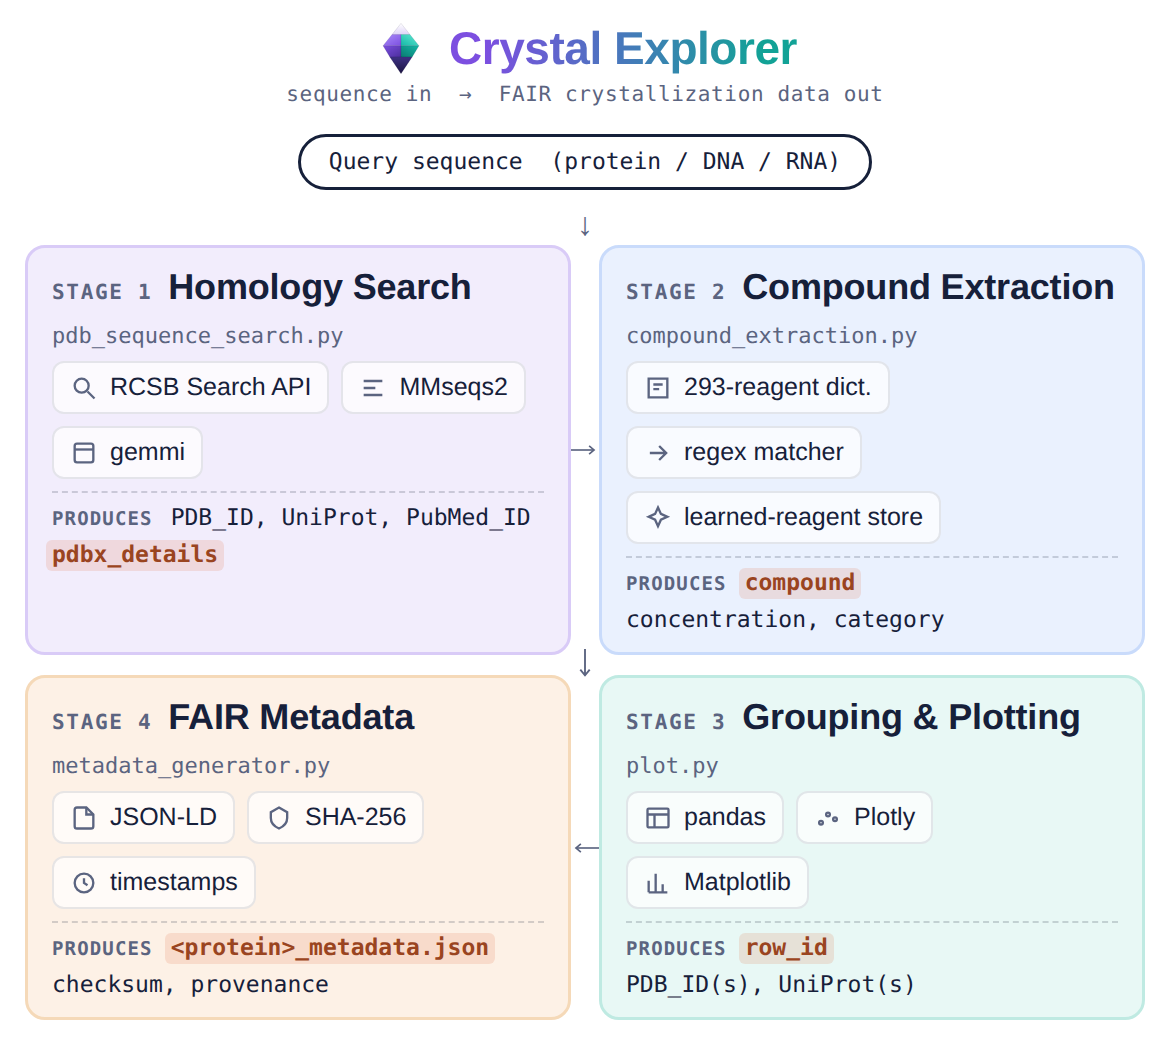
\includegraphics[width=\linewidth]{figures/pipeline_diagram.png}
\caption{Crystal Explorer's four-stage pipeline, from an input sequence to
a FAIR-documented result: each stage's script, the libraries/services it
calls, and the structured fields it hands to the next stage (the one that
stage actually consumes is highlighted). Every stage reads and writes
plain CSV/JSON under a single per-run output directory, so it can also
run standalone from the command line.}
\label{fig:architecture}
\end{figure}

A deliberate design choice is that stages 1 - 4 run on a background
thread spawned by the request handler, which redirects to the results
page immediately; that page polls until the run completes. A run that
can take tens of seconds for larger hit counts; therefore the form
defaults \texttt{max\_hits} to 25.

\subsection{Stage 1: Homology Search and Metadata Retrieval}

Given a sequence, Crystal Explorer builds an RCSB Search API v2 query
combining a sequence similarity node (sequence type, configurable minimum
identity and maximum E-value) with a text filter restricting results to
X-ray entries, at the polymer entity level with full match context per
hit. Hits are deduplicated to one row per PDB entry, keeping the
highest identity match when an entry has several.

For every retained PDB ID, the pipeline fetches the corresponding mmCIF
file (cached after the first download) and parses it with \texttt{gemmi} to
extract the resolution, PubMed ID, UniProt accession(s), polymer type and
assembly, crystallization method, pH, temperature, and the raw
\texttt{pdbx\_details} text with pH, temperature, and method falling
back to a heuristic regex over \texttt{pdbx\_details} when their mmCIF
fields are absent. For a multi-chain complex, the pipeline distinguishes
the UniProt accession that matched the \emph{query} sequence from
bound-partner accessions, so the web UI can bold the query's own rather
than an arbitrary one. Per-hit network calls are issued concurrently
(bounded thread pool) with retry-backoff, and the stage filters its
output to only entries carrying real experimental crystallization
detail.

\subsection{Stage 2: Reagent and Concentration Extraction}

The core difficulty this stage addresses is that
\texttt{pdbx\_details} is free text written independently by thousands of
depositors, with no controlled vocabulary. This is addressed 
with a curated dictionary mapping 354 canonical reagent names to 1{,}180
lexical variants (abbreviations, chemical formulas, alternate spellings,
and unit conventions), spanning PEGs and Jeffamines, inorganic salts,
buffers, organic precipitants, cryoprotectants/additives, detergents,
amino acids, and cofactors, built by mining real \texttt{pdbx\_details}
text across the pipeline's own cache corpus (on the order of
$7.9\times10^3$ entries at the time of writing). Every reagent also
carries a category (Buffer, Salt, Precipitant, or Additive; 30/78/53/124
entries respectively), used downstream to summarize reagent frequency by
role.

\texttt{pdbx\_details} strings are first split into condition clauses
(on commas, semicolons, ``and'', and line breaks, with method keywords
and bare temperature/pH clauses discarded). Each clause is then matched
against the dictionary with three regex patterns applied in order of
specificity: (A) \emph{amount--unit--\allowbreak reagent}, e.g.\ ``0.2~M
ammonium sulfate''; (B) the less common reversed order; and (C) a
bare-reagent fallback recording a known compound with no stated
concentration rather than silently dropping it. Aliases are matched
longest-first and guarded against matching inside an unrelated longer
word; because clause-splitting is itself heuristic, the matcher blanks
out each match's span and re-searches the remainder so a clause can
still yield more than one reagent. Newly encountered reagents can be
registered at runtime, persisted to a learned-reagent store.

\subsection{Stage 3: Grouping, Plotting, and Reporting}

Distinct hits frequently describe the very same crystallization
condition -- e.g.\ several chain copies or space groups of one complex
solved from one crystal. Stage 3 groups rows sharing the same (PubMed
ID, method, pH, extracted-compound signature) key into a single
condition, merging their PDB IDs (and per-entry UniProt accessions) into
one row, and assigns each group a \texttt{row\_id} shared across every
downstream artifact. From the grouped table it produces two scatter
plots -- pH vs.\ temperature and pH vs.\ PEG concentration -- colored by
RCSB relevance score and shaped by method, plus a word-wrapped PDF
summary table. Because Matplotlib output is static, every plotted point
is instead labeled with its PDB ID(s) and \texttt{row\_id}, and a
\texttt{Grouped\_conditions.csv} carrying that same \texttt{row\_id} is
written alongside so the web application  can reconstruct
clickable, linked versions of the same figures.

\subsection{Stage 4: FAIR-Compliant Metadata Generation}

The final stage walks every file the run produced and emits a single
JSON-LD metadata document aligned with the FAIR
principles~\cite{wilkinson2016fair}, recording per file a unique
identifier, MIME type, size, SHA-256 checksum, category, and
human-readable description, and at the dataset level creation
timestamps, software version, author identifiers (including ORCID),
license, and PDB data-source provenance -- automatically, so
reproducibility metadata is a byproduct of using the tool rather than a
separate curation task.

% ============================================================================
\section{Web Application}

The results page renders the pH-vs-PEG and pH-vs-temperature data of
Stage~3 as interactive Plotly figures alongside the full conditions
table, linking a plotted point to its table row via the shared
\texttt{row\_id} (Fig.~\ref{fig:weboverview}). Every identifier in the
table is a live outbound link built from identifiers already attached
during Stages~1-2: \textbf{PDB ID} and \textbf{UniProt} link to RCSB and
UniProt respectively, bolding the accession that matches the query
sequence and color-coding bound-partner accessions from other chains of
a merged complex (\texttt{6XA9}/\texttt{6XAA} each merge the PLpro
chain, P0DTD1, with a different bound partner), \textbf{PubMed} links to
the source publication, and each compound links to PubChem, with a
``3D View'' button loading the structure in an in-page
Mol*~\cite{sehnal2021molstar} viewer (Fig.~\ref{fig:webtable}).

\begin{figure}[t]
\centering
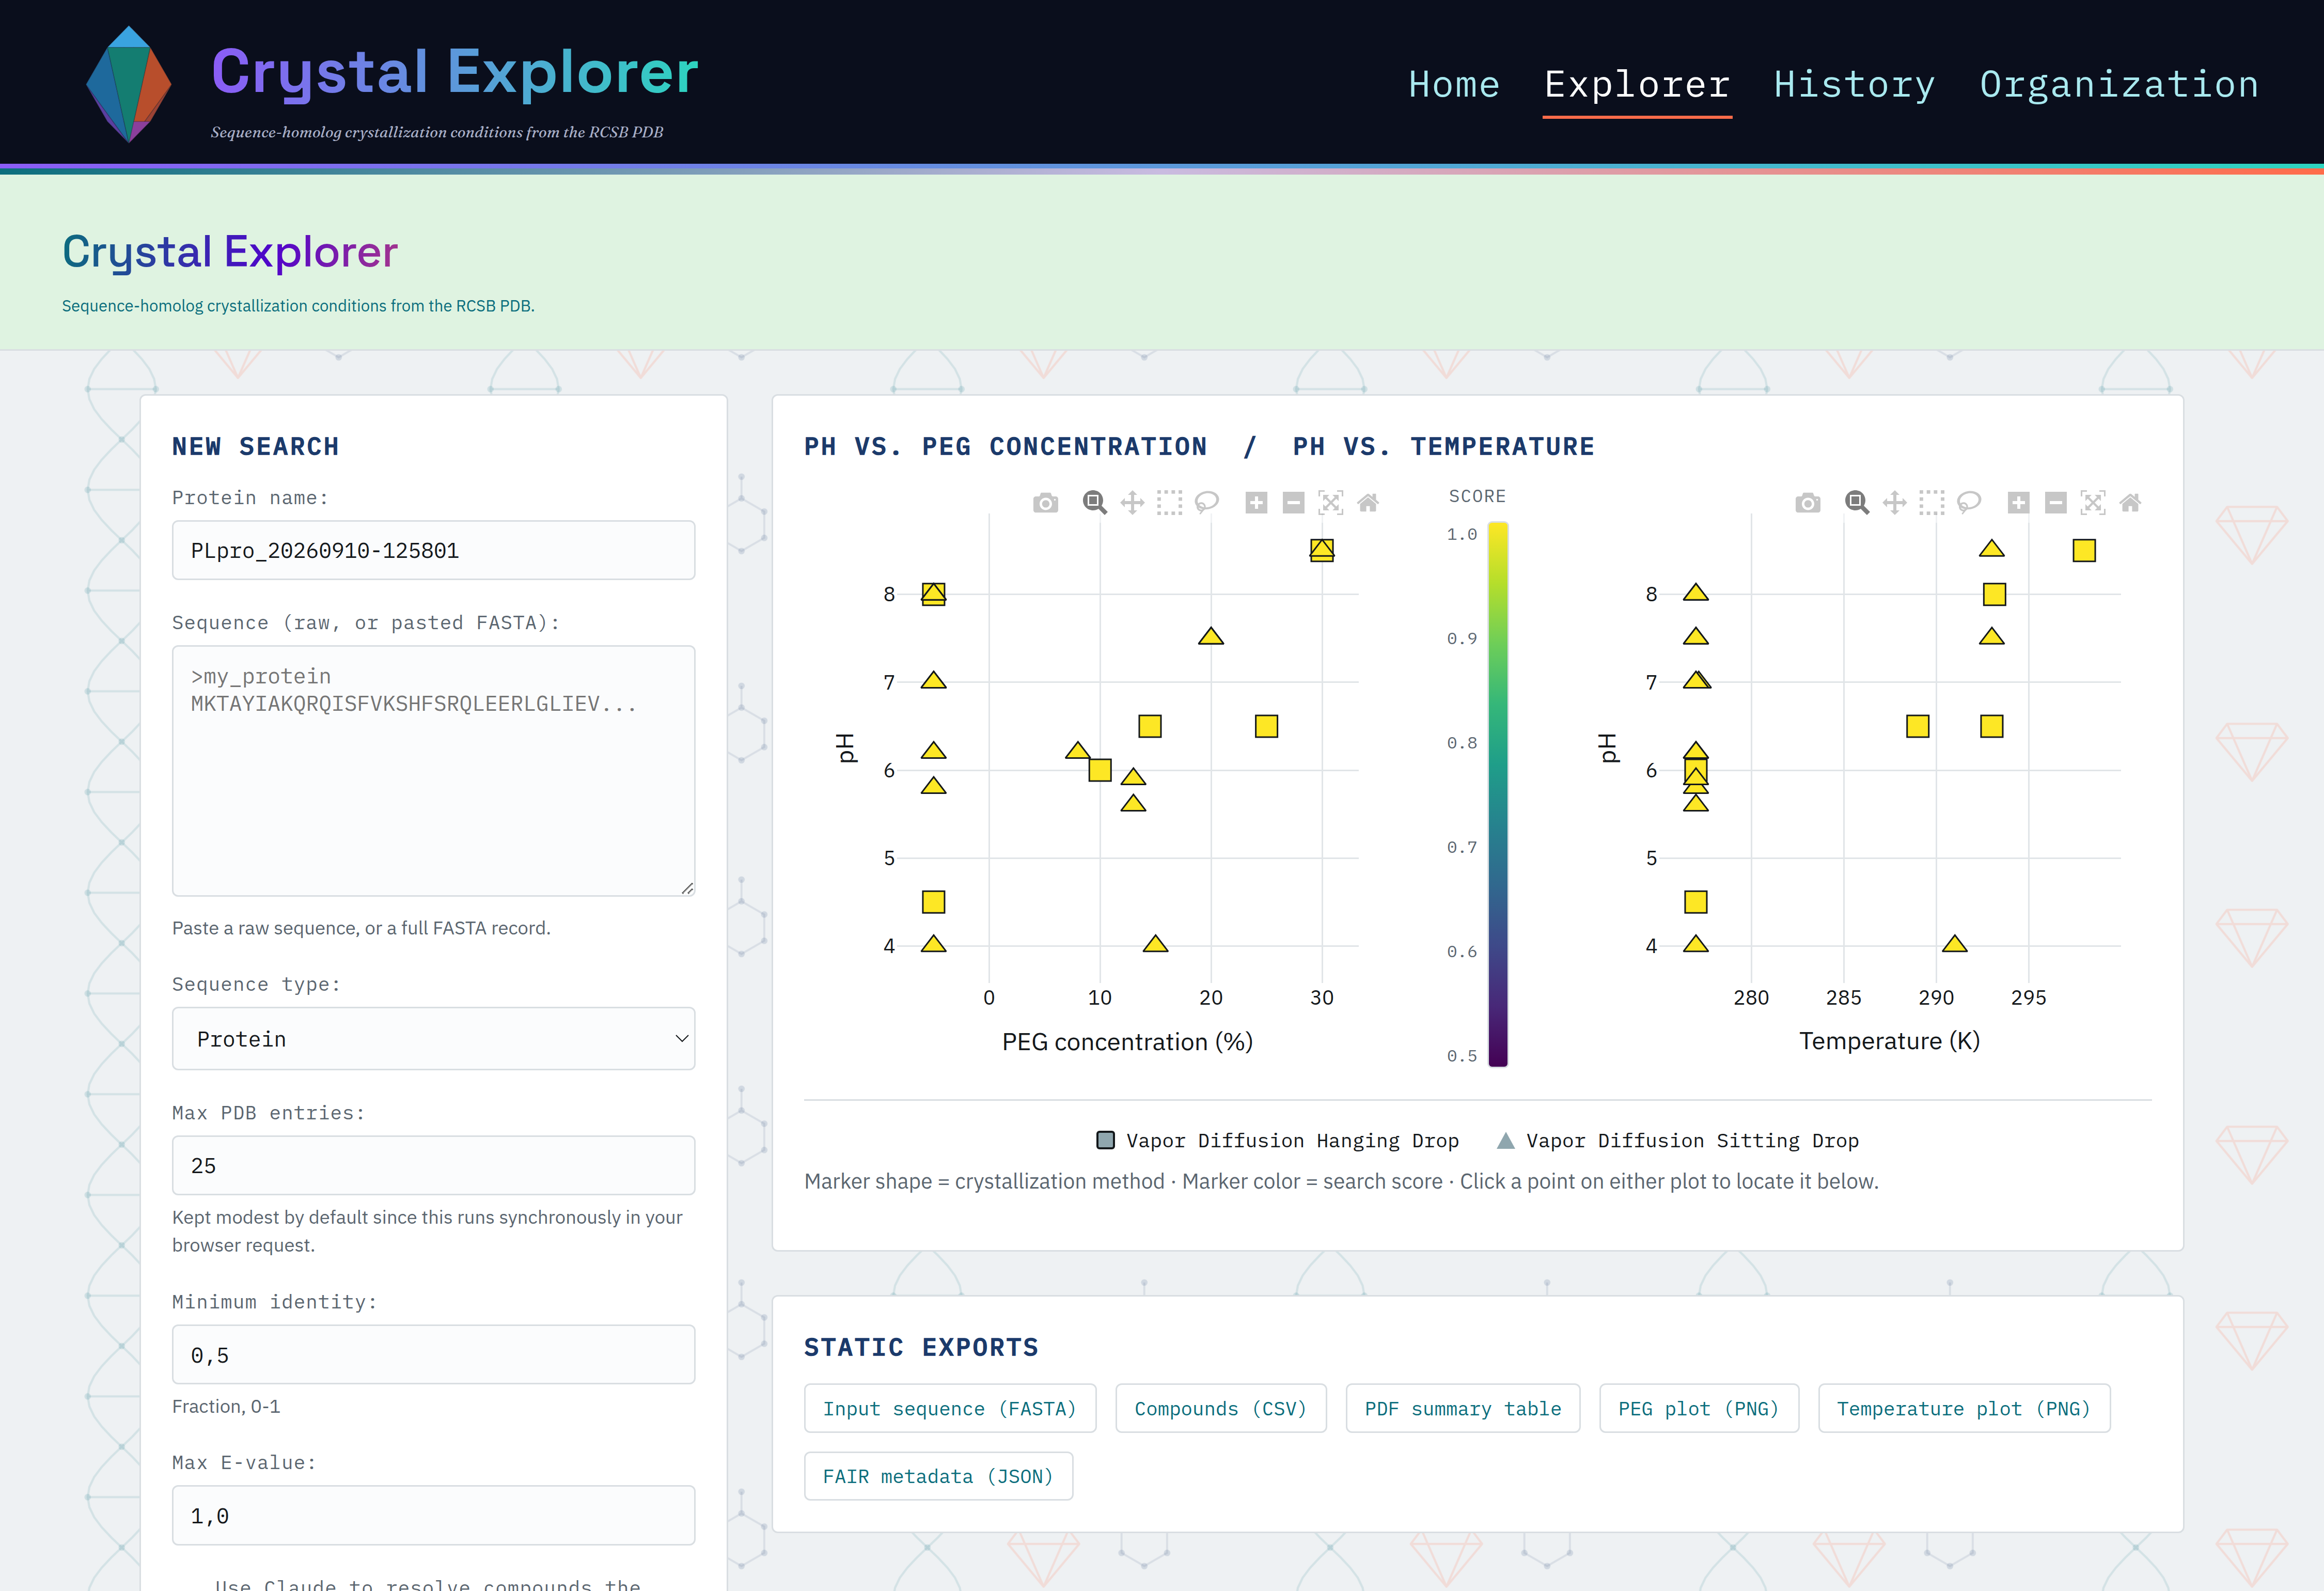
\includegraphics[width=0.92\linewidth]{figures/webapp_after_run_overview.png}
\caption{Crystal Explorer's results page for a real PLpro search: the
search form (left) shows the parameters used, alongside the interactive
pH-vs-PEG and pH-vs-temperature plots and the Static Exports panel of
downloadable artifacts.}
\label{fig:weboverview}
\end{figure}

\begin{figure*}[t]
\centering
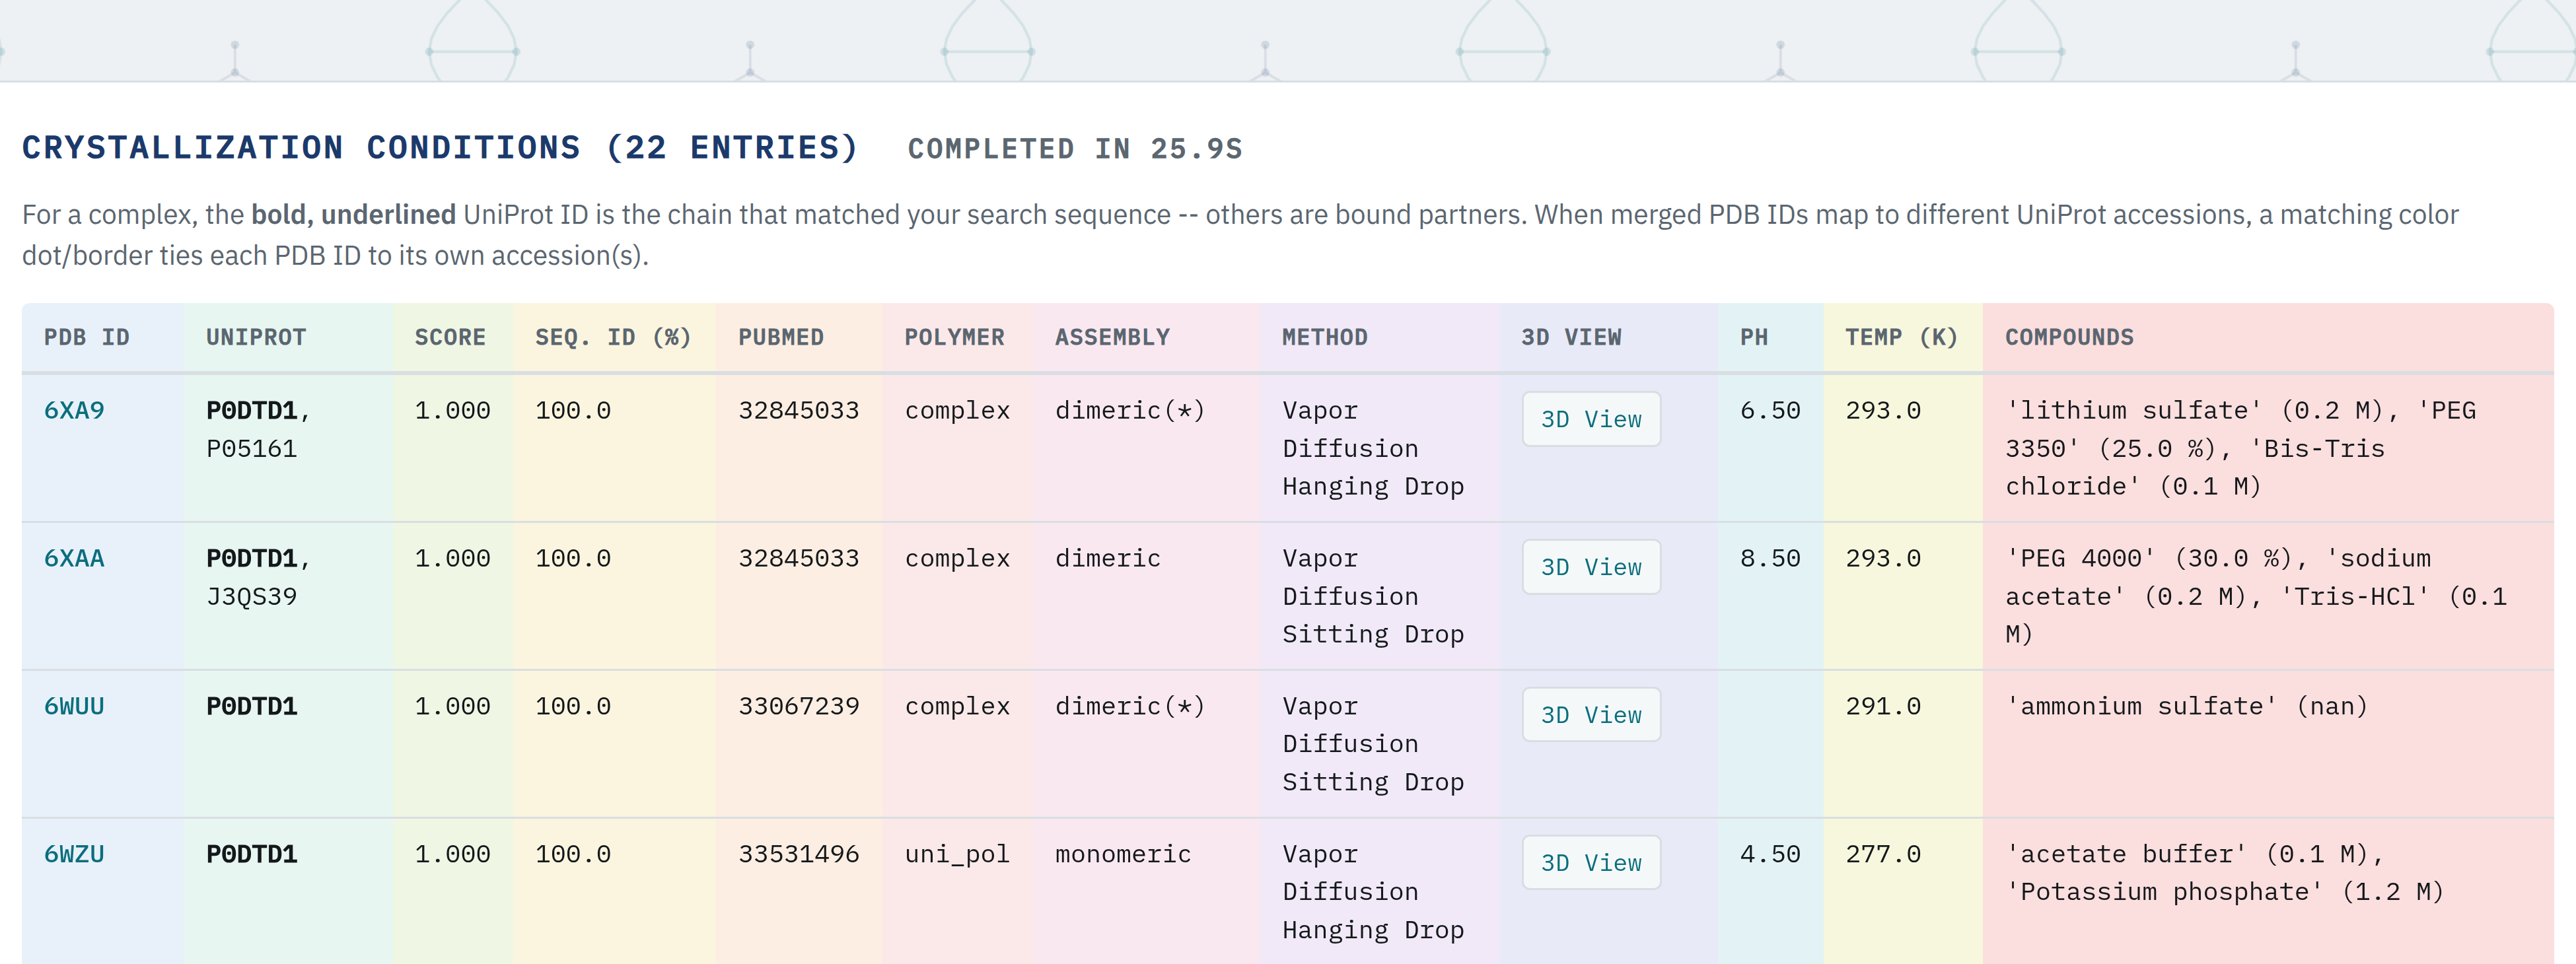
\includegraphics[width=0.92\linewidth]{figures/webapp_conditions_table.png}
\caption{The conditions table for that PLpro search (4 of 22 rows shown;
the on-page table scrolls to reveal the rest). PDB ID and PubMed link out
to RCSB and the source publication; UniProt links to UniProt, bolding the
query-matching accession and color-coding bound-partner accessions in a
merged complex; the Compounds column holds the extracted
cocktail.}
\label{fig:webtable}
\end{figure*}

A reagent-frequency panel further down the same page tallies how often
each dictionary reagent appears across the matched conditions, grouped
by role, so the dominant cocktail components are visible at a glance
rather than read out of the table row by row (Fig.~\ref{fig:webreagent}).

\begin{figure}[t]
\centering
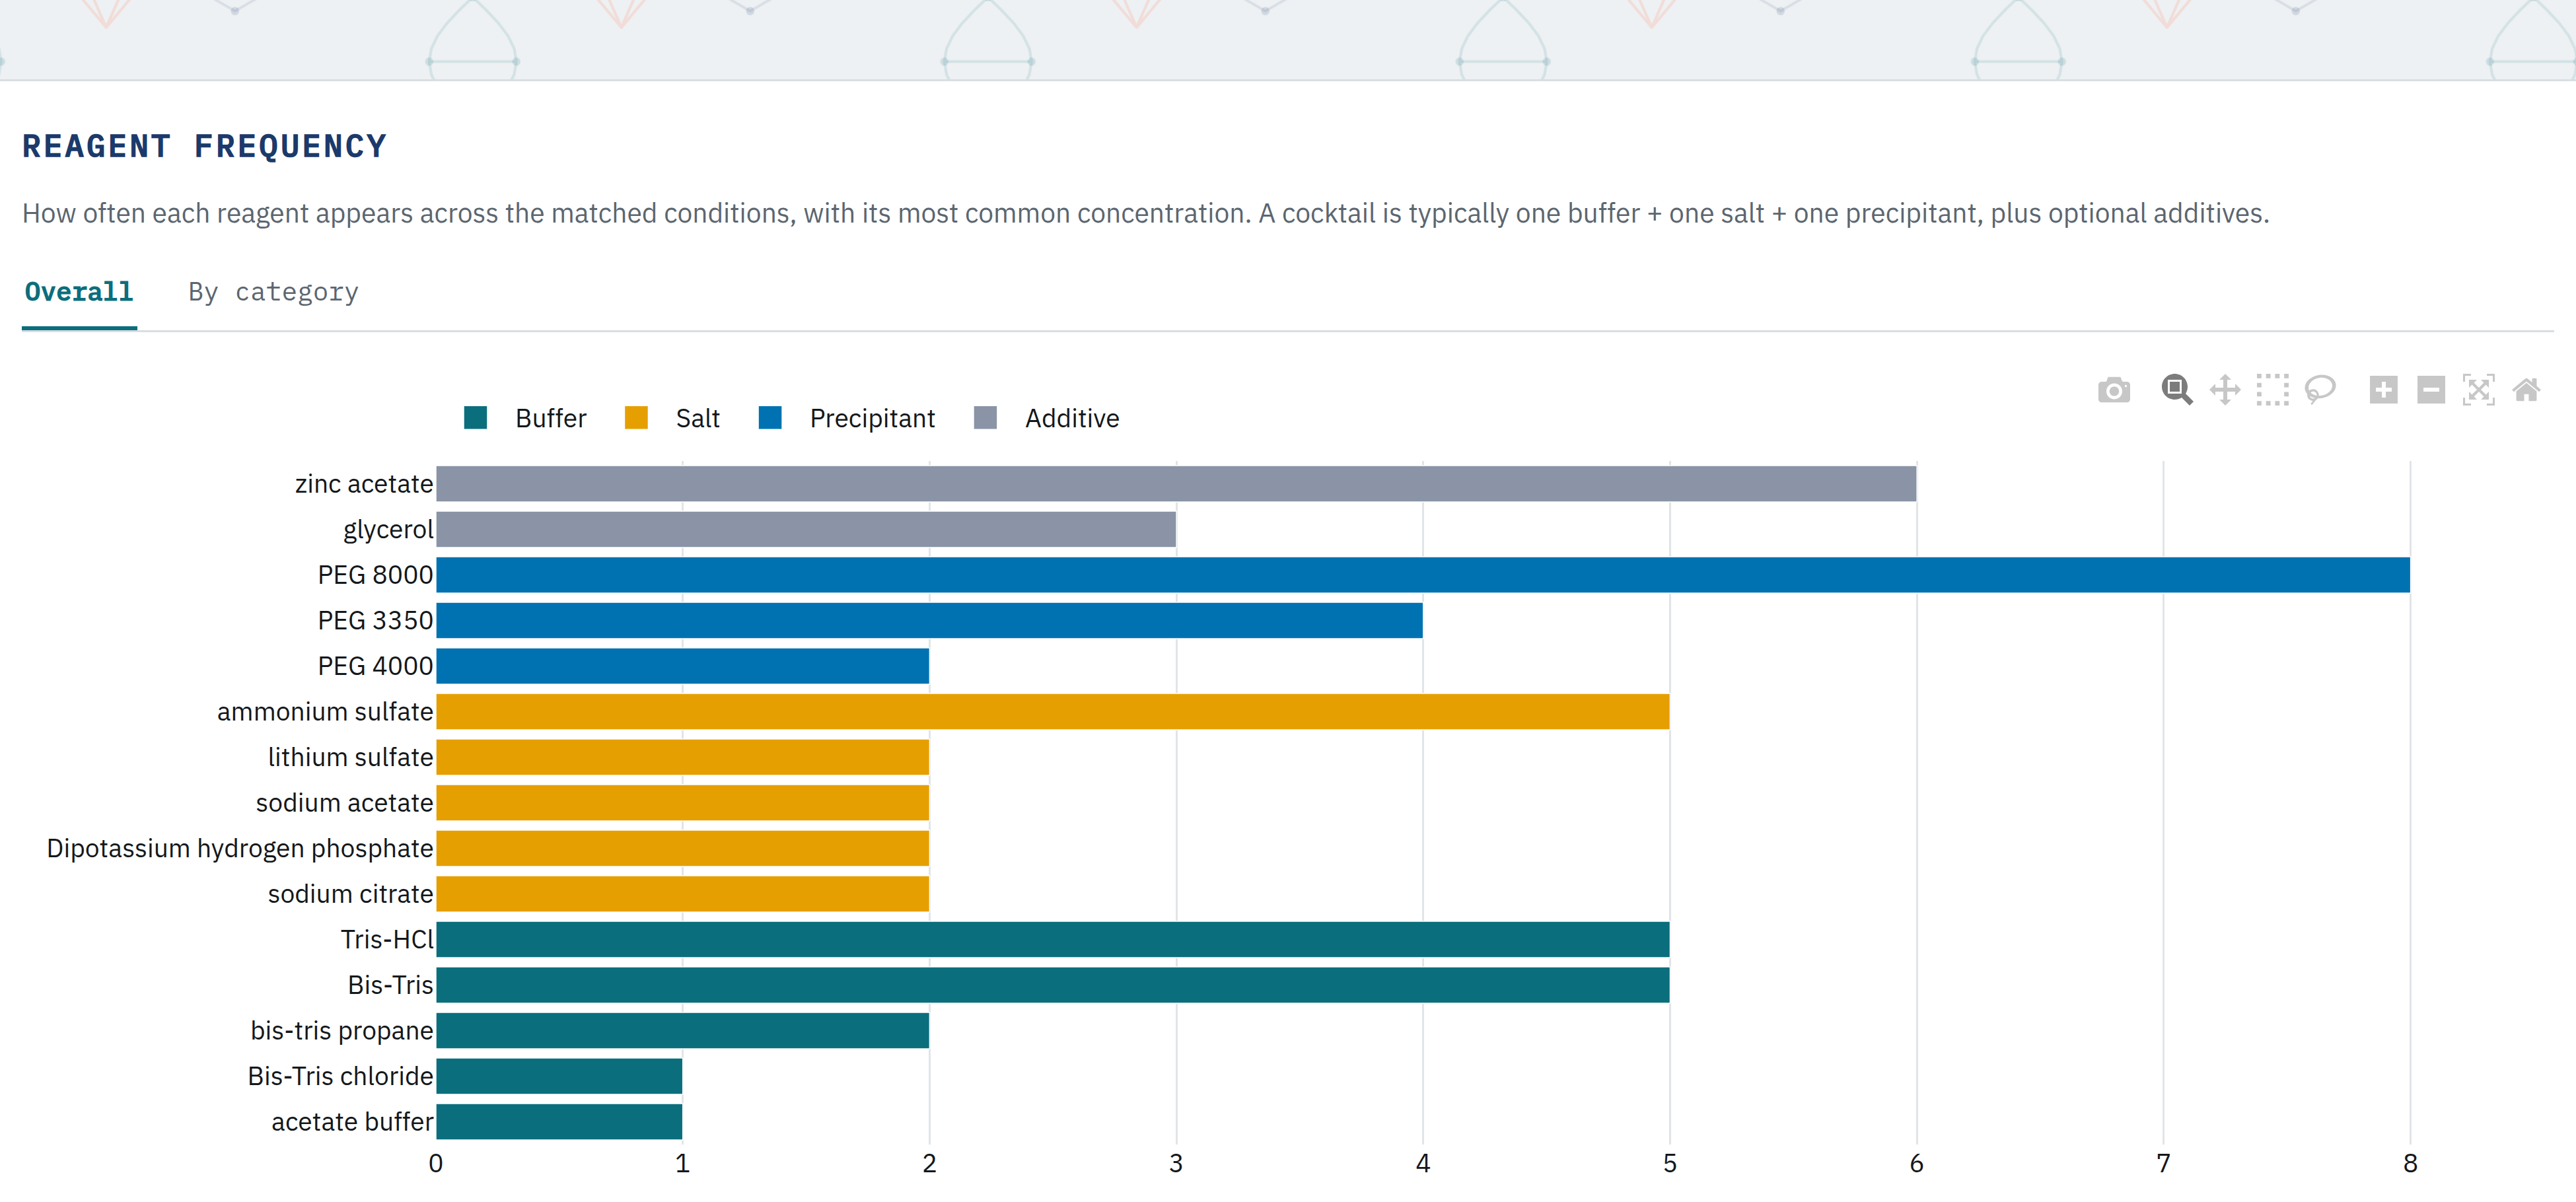
\includegraphics[width=0.92\linewidth]{figures/webapp_reagent_frequency.png}
\caption{Reagent-frequency panel for the same PLpro search: how many
matched conditions use each reagent, colored by role.}
\label{fig:webreagent}
\end{figure}

% ============================================================================
\section{Illustrative Example}

The PLpro search shown in Figs.~\ref{fig:weboverview}--\ref{fig:webreagent}
grounds the pipeline's behavior in a real run rather than a synthetic
example: run with default thresholds ($\geq$50\% identity, E-value
$\leq 1.0$, max hits = 25), it returned 26 X-ray-solved entries,
completing end to end in under 30 seconds. Stage 3 grouped them into the
22 distinct conditions of Fig.~\ref{fig:webtable}; three (PDB entries
7QCM, 7QCI, 7QCG) were merged into a single row since they share the same
publication, method, pH, and extracted cocktail -- e.g.\ ``0.2~M lithium
sulfate, 25\% PEG~3350, 0.1~M Bis-Tris chloride, pH~6.5'' (PDB 6XA9),
correctly decomposed into canonical reagent names with normalized
concentrations and units. This illustrates the pipeline's core value:
instead of reading 26 free-text strings by hand, a researcher targeting a
PLpro-like protease is immediately shown 22 literature-grounded candidate
cocktails, ranked and traceable back to their source structures and
publications.

% ============================================================================
\section{Evaluation}

This section measures how effective \texttt{compound\_extraction.py} --
the dictionary-and-regex extractor described in Section~III-B, with no
LLM involved -- is at pulling structured (compound, concentration) pairs
out of real \texttt{pdbx\_details} text, using the same precision/recall/F1
structure as comparable literature-extraction tools (e.g.\ aTUNApy's LLM
benchmark~\cite{delmoralmorales2026atunapy}).

\subsection{Panels and Protocol}

Two independent evaluation panels of 10{,}000 entries each were built
with the same protocol. Target proteins were drawn at random from
30\%-sequence-identity clusters of X-ray protein entities in the PDB
(60--900 residues, clusters with at least 20 members), one
representative per cluster, so that the panels span many unrelated
protein families rather than a few well-studied ones; neither panel
shares a protein, a cluster or a PDB entry with the PLpro case study of
Section~V, with any earlier test set, or with the other panel. Each
target was run through Crystal Explorer's own pipeline at default
thresholds ($\geq$50\% identity, E-value $\leq 1.0$, hit cap 30), and
every retained hit with a non-empty \texttt{pdbx\_details} field joined
a pool of unique entries, from which 10{,}000 were drawn at random.
A random 1{,}000 of each panel were then audited by hand, in twenty
batches of 50: for every entry the raw text was read, the true reagent
list written down, and the extractor's output scored against it, with a
note explaining every error.

Scoring is per distinct reagent per entry. A ground-truth reagent is a
true positive (TP) if reported, under its own name or a name of the
right chemical family (e.g.\ a generic ``PEG'' for ``polyethylene glycol
8{,}000''), and a false negative (FN) if missed; a reported compound that
is a \emph{different} chemical from the one in the text (``PEG 5000'' for
``PEG 5000 MME'', ``ATP'' for ``$\alpha,\beta$-methylene-ATP'') counts as
one FP and one FN. Proteins and peptides, unnamed ligands (``inhibitor'',
``compound 4''), named commercial mixes with no listed components, and
pH titrants are excluded; concentrations are not scored. A stricter
entry-level accuracy credits an entry only if it has zero misses
\emph{and} zero false positives. The audit was carried out by a single
annotator, and 95\% confidence intervals were obtained by bootstrap
resampling of entries (5{,}000 resamples).

The first panel (505 targets, a pool of 10{,}153 entries) served as a
\emph{development} set: the abbreviations, typos and formatting cases its
audit exposed were fixed afterwards, changing the output on 428 entries.
The second panel (683 targets, a pool of 14{,}145 entries) is the
\emph{held-out} test of that fixed extractor. Its samples were drawn
only after the fixes, the extractor's SHA-256 hash was recorded when they
were drawn, and it was verified to be unchanged once the last batch was
scored, so no part of the extractor was tuned on this panel. Both
panels, their audited samples, the per-entry annotations, and the
scripts used to build them and compute the metrics below are published
in the project's GitHub repository.

\subsection{Results}

Table~\ref{tab:heldout} reports both audits. On the held-out panel the
extractor reaches 99.3\% precision and 94.2\% recall (F1 0.967), and
84.6\% of entries are extracted without a single error. Compared with
the development panel, recall rose by 1.5 points and entry-level
accuracy by 3.0 points while precision was unchanged; the confidence
intervals of the two panels overlap only slightly, consistent with a
modest but real gain from the fixes, measured on proteins the extractor
had never been tuned on. Over the whole held-out panel, without ground
truth, 95.1\% of the 10{,}000 entries yield at least one compound
(2.81 per entry on average, 305 distinct compounds), and 82.1\% of the
extracted compounds carry a concentration.

\begin{table}[t]
\centering
\caption{Extraction effectiveness of \texttt{compound\_extraction.py} on
1{,}000 manually audited entries from each of two independent
10{,}000-entry panels of real PDB data. 95\% bootstrap confidence
intervals in brackets.}
\label{tab:heldout}
\setlength{\tabcolsep}{4pt}
\begin{tabular}{lcc}
\toprule
 & Development & \textbf{Held-out} \\
 & (before fixes) & \textbf{(fixed, frozen)} \\
\midrule
Target proteins & 505 & 683 \\
Audited entries & 1{,}000 & 1{,}000 \\
Ground-truth mentions & 3{,}031 & 2{,}898 \\
True positives & 2{,}810 & 2{,}731 \\
False positives & 23 & 20 \\
False negatives & 221 & 167 \\
\midrule
Precision & 0.992 & \textbf{0.993} \\
 & {\footnotesize[0.988, 0.995]} & {\footnotesize[0.989, 0.996]} \\
Recall & 0.927 & \textbf{0.942} \\
 & {\footnotesize[0.917, 0.937]} & {\footnotesize[0.934, 0.951]} \\
F1 & 0.958 & \textbf{0.967} \\
 & {\footnotesize[0.952, 0.964]} & {\footnotesize[0.962, 0.972]} \\
Entry-level accuracy & 0.816 & \textbf{0.846} \\
 & {\footnotesize[0.792, 0.840]} & {\footnotesize[0.824, 0.868]} \\
\bottomrule
\end{tabular}
\end{table}

\subsection{Error Analysis}

The 20 false positives of the held-out panel are almost all a related
but \emph{different} compound rather than an invented one. Four are a
PEG monomethyl ether reported as plain PEG when ``MME'' is written in an
unusual position (``PEG 5K monomethylether'', ``MONOMETHYL-PEG 5000'');
three are glycyl-glycyl-glycine reported as glycylglycine; and several
are a modified compound cut down to the shorter name it contains
(pyridoxal-5$'$-phosphate as ``phosphate'', deaza-PLP as PLP,
myristoyl-CoA as coenzyme~A, 2-fluoro-cellotriose as cellotriose). The
rest are single cases, such as potassium cacodylate reported as the
sodium salt. The 167 false negatives fall into three groups. The largest
is an open-ended tail of small-molecule ligands, inhibitors and soaking
compounds with no dictionary entry at all -- opaque compound codes
(HGN-1310, IMP-1002, L742001), drugs (gefitinib, pelitinib), nucleotides
and sugars (cAMP, ddCTP, UDP-galactose), and metabolites such as
2-oxoglutarate -- the same long-tail pattern seen in the development
panel. The second is reagents that are common enough to deserve an
entry but did not yet have one (succinic acid, guanidine, ethanolamine,
sodium oxalate, triethylene glycol, 18-crown-6). The third is
abbreviations and depositor typos a literal-alias dictionary cannot
anticipate (``NA BR'', ``CH3COONA'', ``PEG 5KMME'', ``Imidanzol'',
``AMMONIUMS SULFATE'', ``Sodiumcitrate''). None of these were fixed while
the panel was being scored, since its purpose is to measure the
extractor as it stands. Precision stayed at 0.99 on both panels --
the extractor rarely reports a compound that is not in the text --
while recall is capped by exactly the open-ended long tail that
Section~VII argues no static dictionary fully closes.

% ============================================================================
\section{Discussion, Limitations, and Future Work}

Crystal Explorer's central relevance to protein crystallization is that
it turns a resource every structural biologist already trusts -- prior,
experimentally successful conditions for a homologous structure -- into
something usable at the moment it matters: before the first screen is
set up. Sparse-matrix screening~\cite{jancarik1991sparse} remains the default starting point
precisely because no comprehensive theoretical model of crystallization
exists~\cite{kwon2013modeling,mcphersoncudney2014optimization}, so a
target with no obviously similar solved structure has little choice but
to sample broadly and expensively across reagent space, often consuming
scarce, hard-to-produce protein before a single hit. When a homolog has
already been crystallized, its recorded condition is a strong empirical
prior for a new, related target -- not a guarantee that the same
cocktail will reproduce a diffraction-quality crystal, since sequence
similarity does not ensure identical crystallization behavior, but a
starting point grounded in a real, successful precedent rather than a
blind guess across reagent space. Retrieving that precedent efficiently
from decades of free-text deposition notes is itself a real, largely
unautomated bottleneck. This is the gap Crystal Explorer closes, for a working
crystallographer rather than a bioinformatician: no local database, no
script, a sequence and a browser. This is not just a promise: on the
held-out panel of Section~VI, 99.3\% of the reagents the extractor
reports are correct and it recovers 94.2\% of the true chemistry a
homolog's record actually contains, so what reaches the
results page is already close to what a human would transcribe by hand.
Because the underlying resource is the PDB itself rather than a
separately maintained screen catalog, the prior also grows automatically
as the field deposits more structures, and every suggested condition
stays traceable back to the structure and publication that reported it
(Section~IV) -- an auditable provenance a sparse-matrix screen cannot
offer.

An important caveat comes from Abrahams and
Newman~\cite{abrahams2019blasting}, who compared sequence similarity
with cocktail similarity across the PDB and found that proteins with
similar but non-identical sequences were crystallized in conditions no
more alike than those of unrelated proteins -- plausibly because crystal
contacts are made by surface residues, which are exactly the residues
that diverge first between homologs. Taken at face value, this argues
against treating a homolog's cocktail as a recipe to copy, and Crystal
Explorer does not present it as one. Its usefulness rests on weaker
claims that this finding leaves intact. First, at the default identity
threshold ($\geq$50\%) many hits are not distant relatives but the same
protein crystallized again -- other constructs, mutants, or ligand
complexes -- and whether the lack of correlation extends to that
near-identical end was not the question we tested. Second, the results
page summarizes the \emph{distribution} of reagents, pH, temperature
and PEG concentration across all retrieved structures, delimiting a
region of chemical space to sample first rather than prescribing a
single condition. Third, every suggestion stays traceable to its
structure and publication, so the user can judge for themselves how
close a construct or ligand state is to their own. Whether
homology-ranked conditions actually raise hit rates over a generic
sparse-matrix screen is an empirical question this work does not
answer; testing it against wet-lab screening outcomes, ideally using the
shared success-and-failure screening data called for by Newman et
al.~\cite{newman2012need}, is the validation this approach still needs.

Two main limitations follow from the design choices above. First,
extraction is heuristic: the held-out evaluation (Section~VI)
reaches 99.3\% precision but 94.2\% recall and 84.6\%
entry-level exact-match accuracy, with a long tail of ligands,
abbreviations and rare reagents a hand-curated dictionary must keep
absorbing, so manual spot-checking remains advisable. The audit itself
was carried out by a single annotator. Second, the pipeline now runs on a
background thread rather than inside the search request itself, which
keeps the UI responsive for one user, but a single in-process thread
pool still does not scale across concurrent users or multiple server
processes; a real task queue (Celery, Django-Q) is the natural next
step if deployment grows past a single \texttt{runserver} process.

A natural next step for closing that recall gap -- not yet
implemented, and worth putting in perspective rather than treating as
an assumed fix -- is an LLM-assisted fallback for reagents the
dictionary comes back empty on. The 167 false negatives of the held-out
panel in Section~VI are overwhelmingly reagents the dictionary simply has no
entry for -- exactly the open-ended, long-tail failure mode a
general-purpose language model is better suited to than an
ever-growing hand-curated alias list, and unlike the buffer-family
mislabelings behind most false positives, a missed entry costs nothing
to leave to a fallback that only runs when the dictionary comes back
empty. Against that, an LLM call adds latency, an external API
dependency, and its own new failure mode -- a plausible-sounding but
wrong compound name -- that the deterministic dictionary does not have,
and which regex matching alone cannot catch. We have not wired it in or
measured it against our own ground truth, so its actual effect on
Table~I's numbers is unknown; aTUNApy's precision above 0.98 and recall
of 0.95 extracting compound mentions from PubMed abstracts with
Claude~\cite{delmoralmorales2026atunapy} -- a different domain and
extraction target from \texttt{pdbx\_details} -- is at best suggestive
that LLM-assisted extraction can reach usable accuracy on comparably
messy chemical text, not evidence that it will transfer here.

Beyond extraction quality, we have not yet
compared condition rankings against validated screens, nor combined this
mining with crystallizability predictors such as
DeepCrystal~\cite{elbasir2019deepcrystal} -- both natural next steps.

% ============================================================================
\section{Conclusion}

We presented Crystal Explorer, an open-source web pipeline that automates
the retrieval, extraction, grouping, and FAIR-compliant documentation of
protein crystallization conditions from homologous X-ray structures,
turning an unstructured, per-entry free-text field into a structured,
literature-grounded shortlist of candidate cocktails through a single
web form. On a held-out panel of 10{,}000 PDB entries, never used to
tune it, a 1{,}000-entry manual audit against 2{,}898 verified reagent
mentions gives 99.3\% precision and 94.2\% recall (F1 0.967),
showing that ligands, rare reagents and source-text typos remain an
open long tail rather than a closed list. The system is released under the MIT license, intended
to lower the barrier to using the PDB's accumulated crystallization
knowledge as a practical starting point for new screens.

% ============================================================================
\section*{Acknowledgment}
The authors would like to acknowledge the support of the administrative
personnel, particularly the staff of the Laboratory of Data Engineering
(LADE) at the Research and Technology Institute (RIT), Area Science Park,
Trieste. 

% ============================================================================
\bibliographystyle{IEEEtran}
\bibliography{references}

\end{document}

